\section{方法描述}

\subsection{图文实体}
\label{sec:4_entities}
\begin{figure}[!htbp]
    \centering
    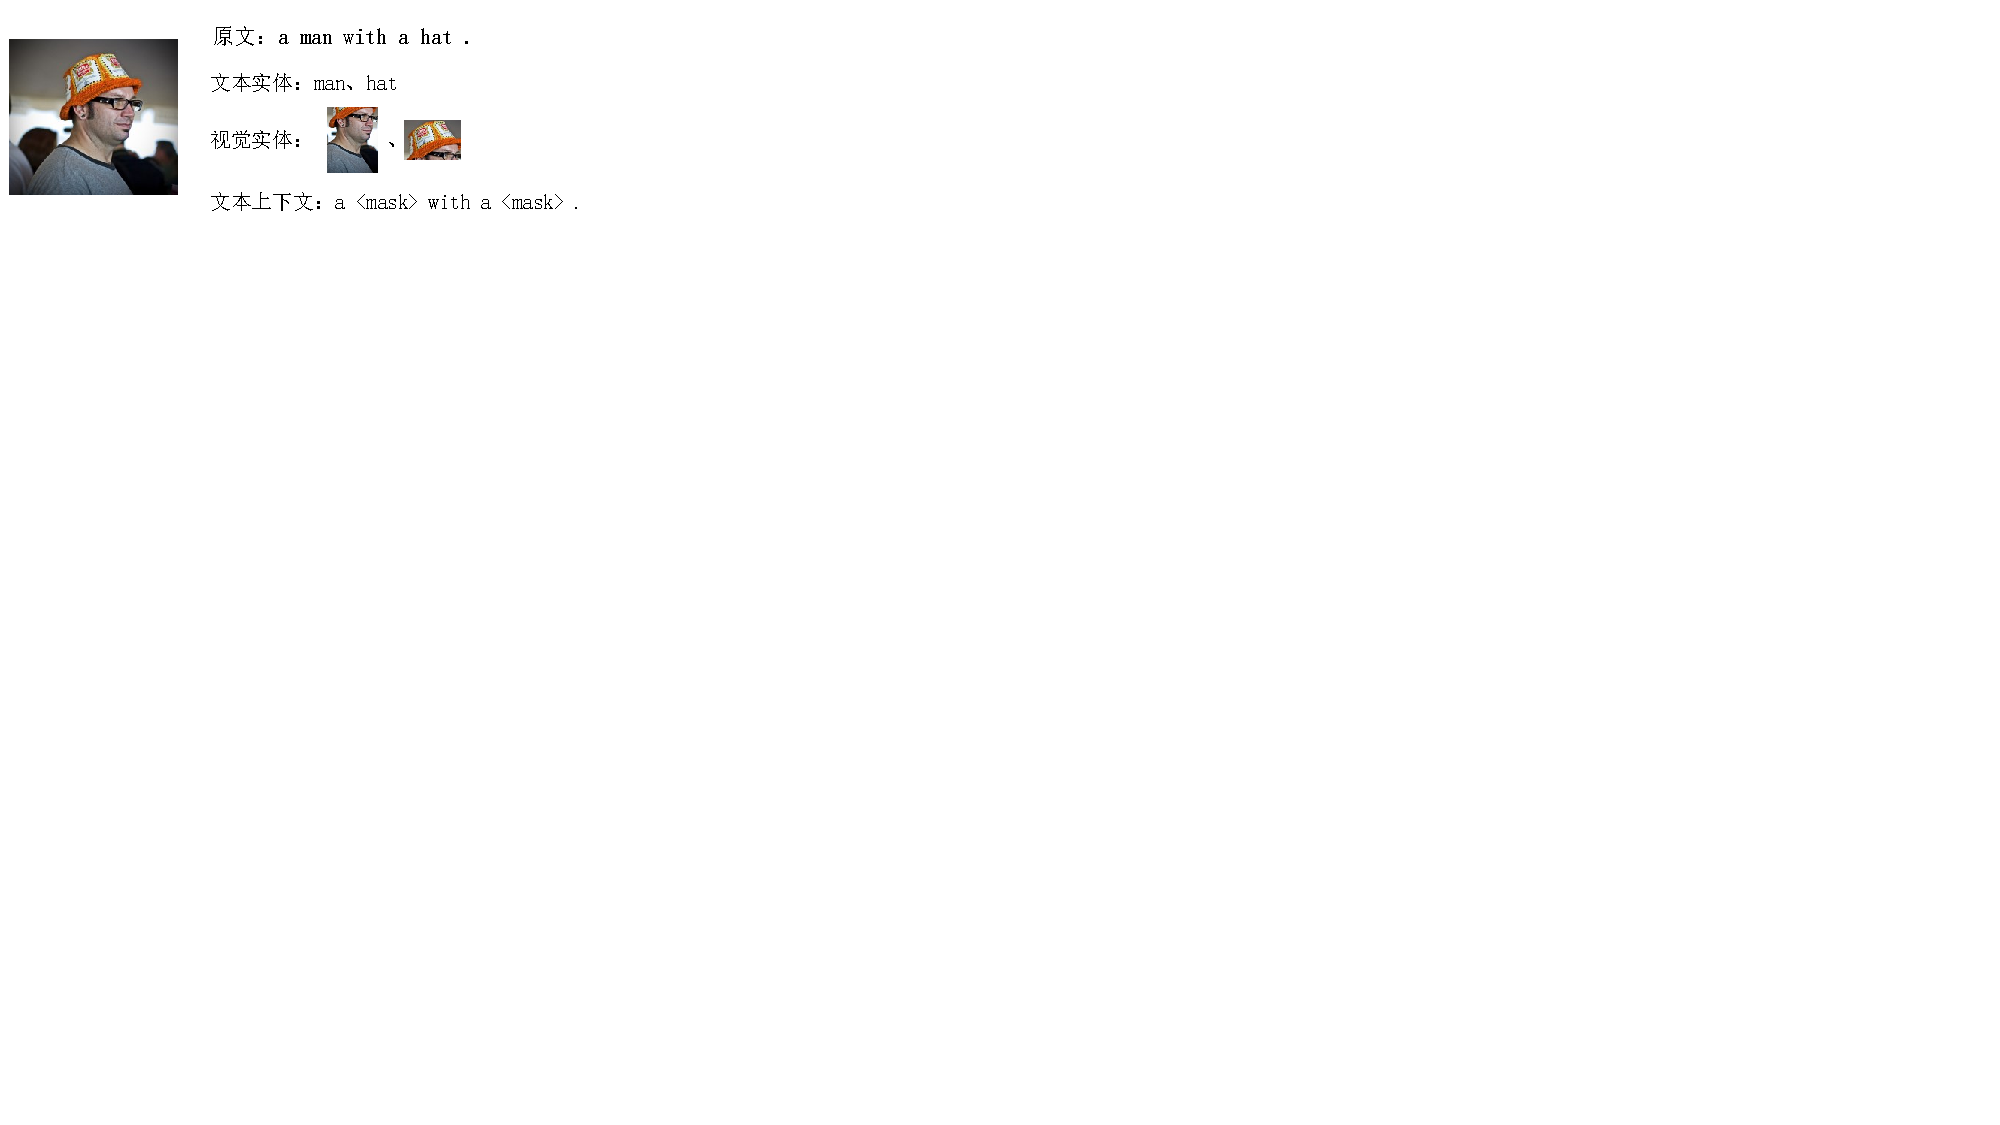
\includegraphics{Img/fig_4_definations.pdf}
    \bicaption{图文实体}{Visual and textual entities}
    \label{fig:4_definations}
\end{figure}
为了更方便地对本章所提CER方法进行介绍,首先需要对CER方法作用到的视觉目标和文本中的作用目标进行更恰当的定义:

(1){\sffamily 文本实体:}输入的源语言句子$X=\{x_1,x_2,\cdots,x_N\}$中,$x_i$代表句子中的每个单词,在句子的对应图片中有对应视觉目标的名词$t_a=x_a,t_b=x_b,\cdots$为文本实体(textual entity),$T=\{t_a,t_b,\cdots\}$为它们的集合,可见$T \subseteq X$。如图\ref{fig:4_definations}所示,名词“man”和“hat”在图片中均有与其对应的视觉目标,因此符合文本实体的定义。从该定义同样可知,文本实体与上一章\ref{sec:3_entity_replacement}小节所介绍的词实体本质上是相同的。本章不再将名词短语划为实体范畴进行考虑,只针对名词融合视觉信息。

(2){\sffamily 视觉实体:}文本实体在对应图片$I$中的对应视觉目标$v_a,v_b,\cdots$为视觉实体(visual entity),$V=\{v_a,v_b,\cdots\}$为它们的集合。图\ref{fig:4_definations}中的“男人”和“帽子”分别是文本实体“man”和“hat”在图片中对应的视觉目标,因此是视觉实体。

(3){\sffamily 文本非实体:}在源语言句子中,所有不是文本实体的单词均可称为文本非实体(textual none-entity)。$\tilde{X}=X-T$代表它们的集合、文本上下文或退化文本。例如图\ref{fig:4_definations}中,文本上下文中除了特殊单词“<mask>”均为文本非实体。

%\subsection{跨模态编码}
%\label{sec:4_cross_modal_encoding}
%\begin{figure}[!htbp]
    \centering
    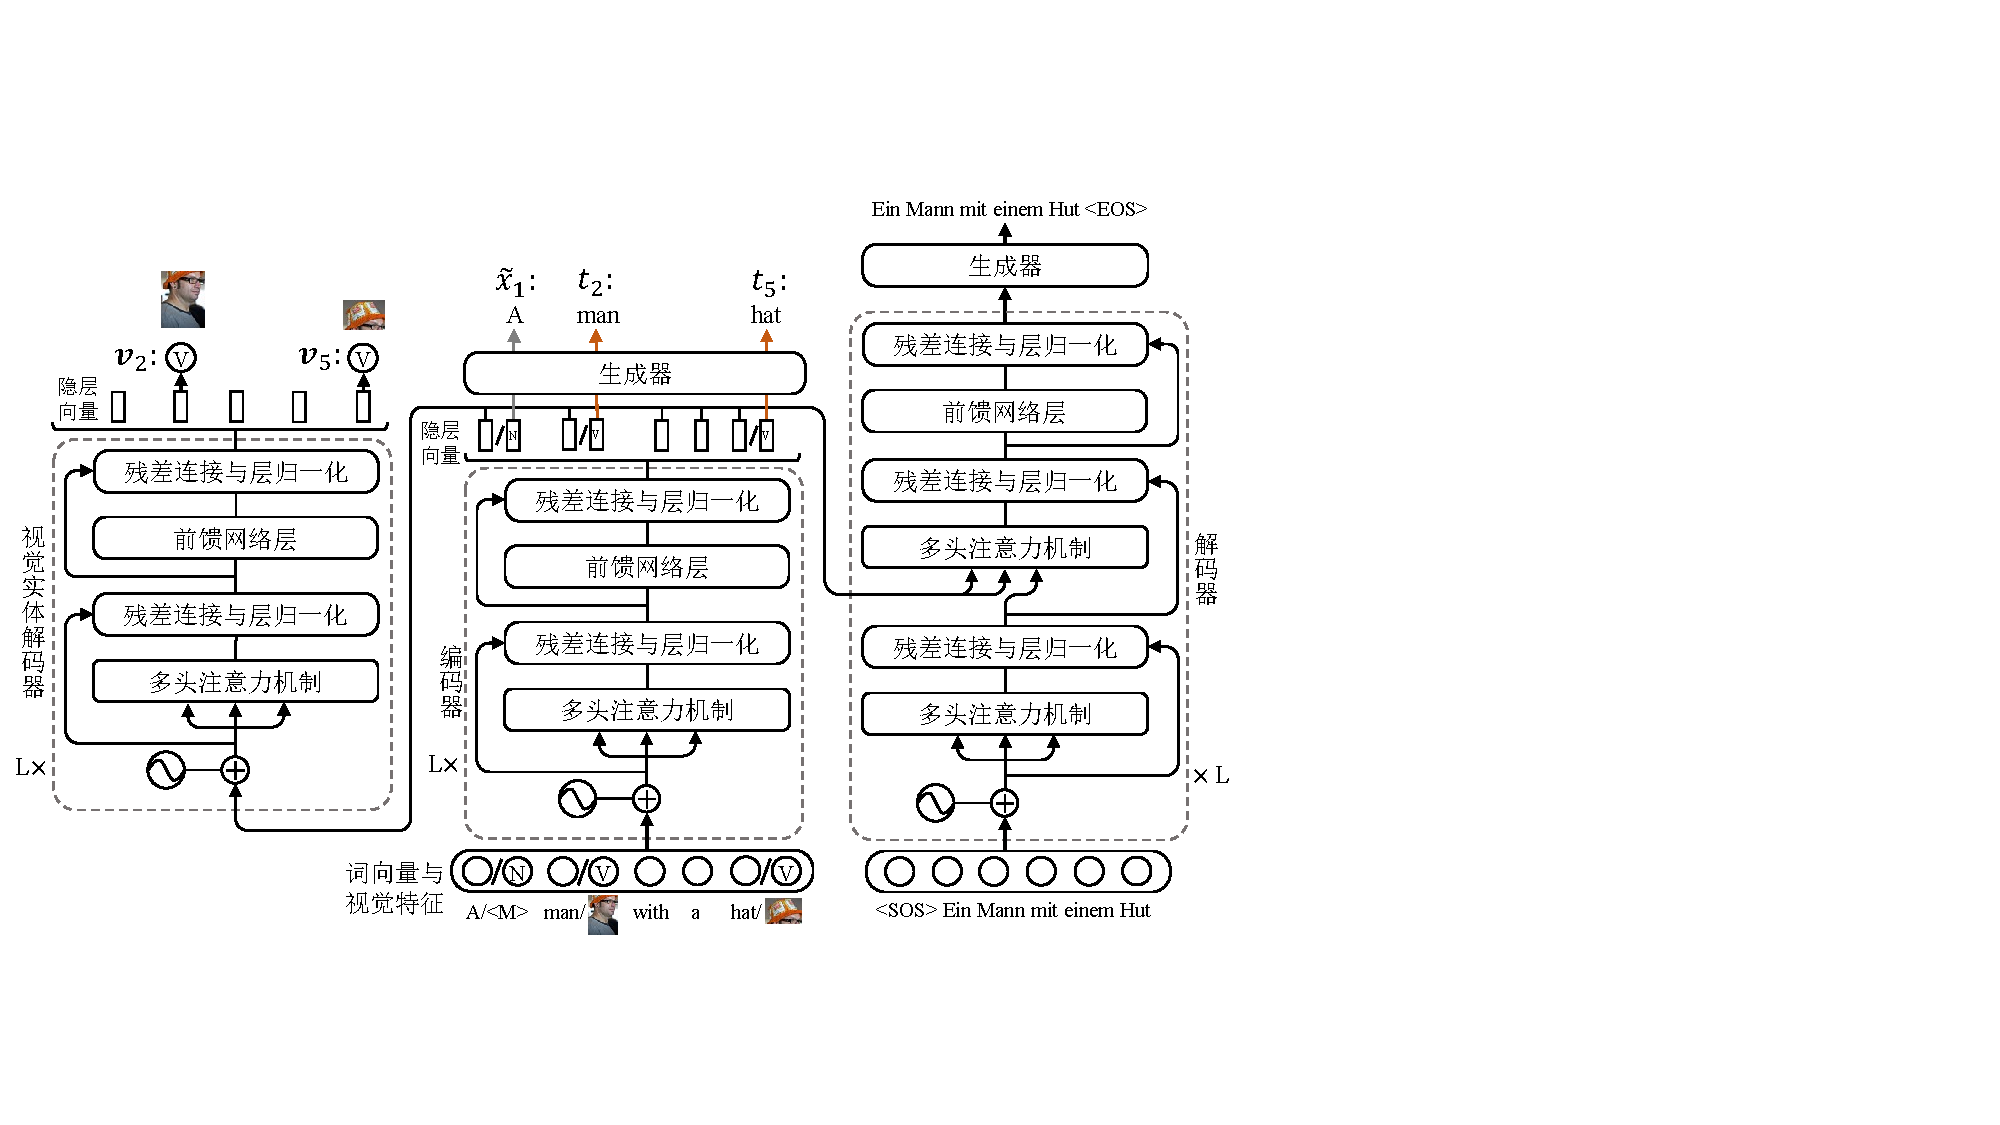
\includegraphics[scale=0.65]{Img/fig_4_model.pdf}
    \bicaption{结合跨模态实体重构方法的神经机器翻译}{NMT model framework combined with CER}
    \label{fig:4_model}
\end{figure}
%图\ref{fig:4_model}展示了CER模型与NMT模型相融合的简化过程,其中包含了视觉实体解码器、跨模态编码器以及翻译解码器三个主要组成部分。其中最核心的跨模态编码器负责在实体重构之前将视觉信息与文本信息编码融合。所编码的信息包含着实体重构主要依赖的三部分:

%\begin{itemize}
%\item
%\begin{figure}[!htbp]
    \centering
    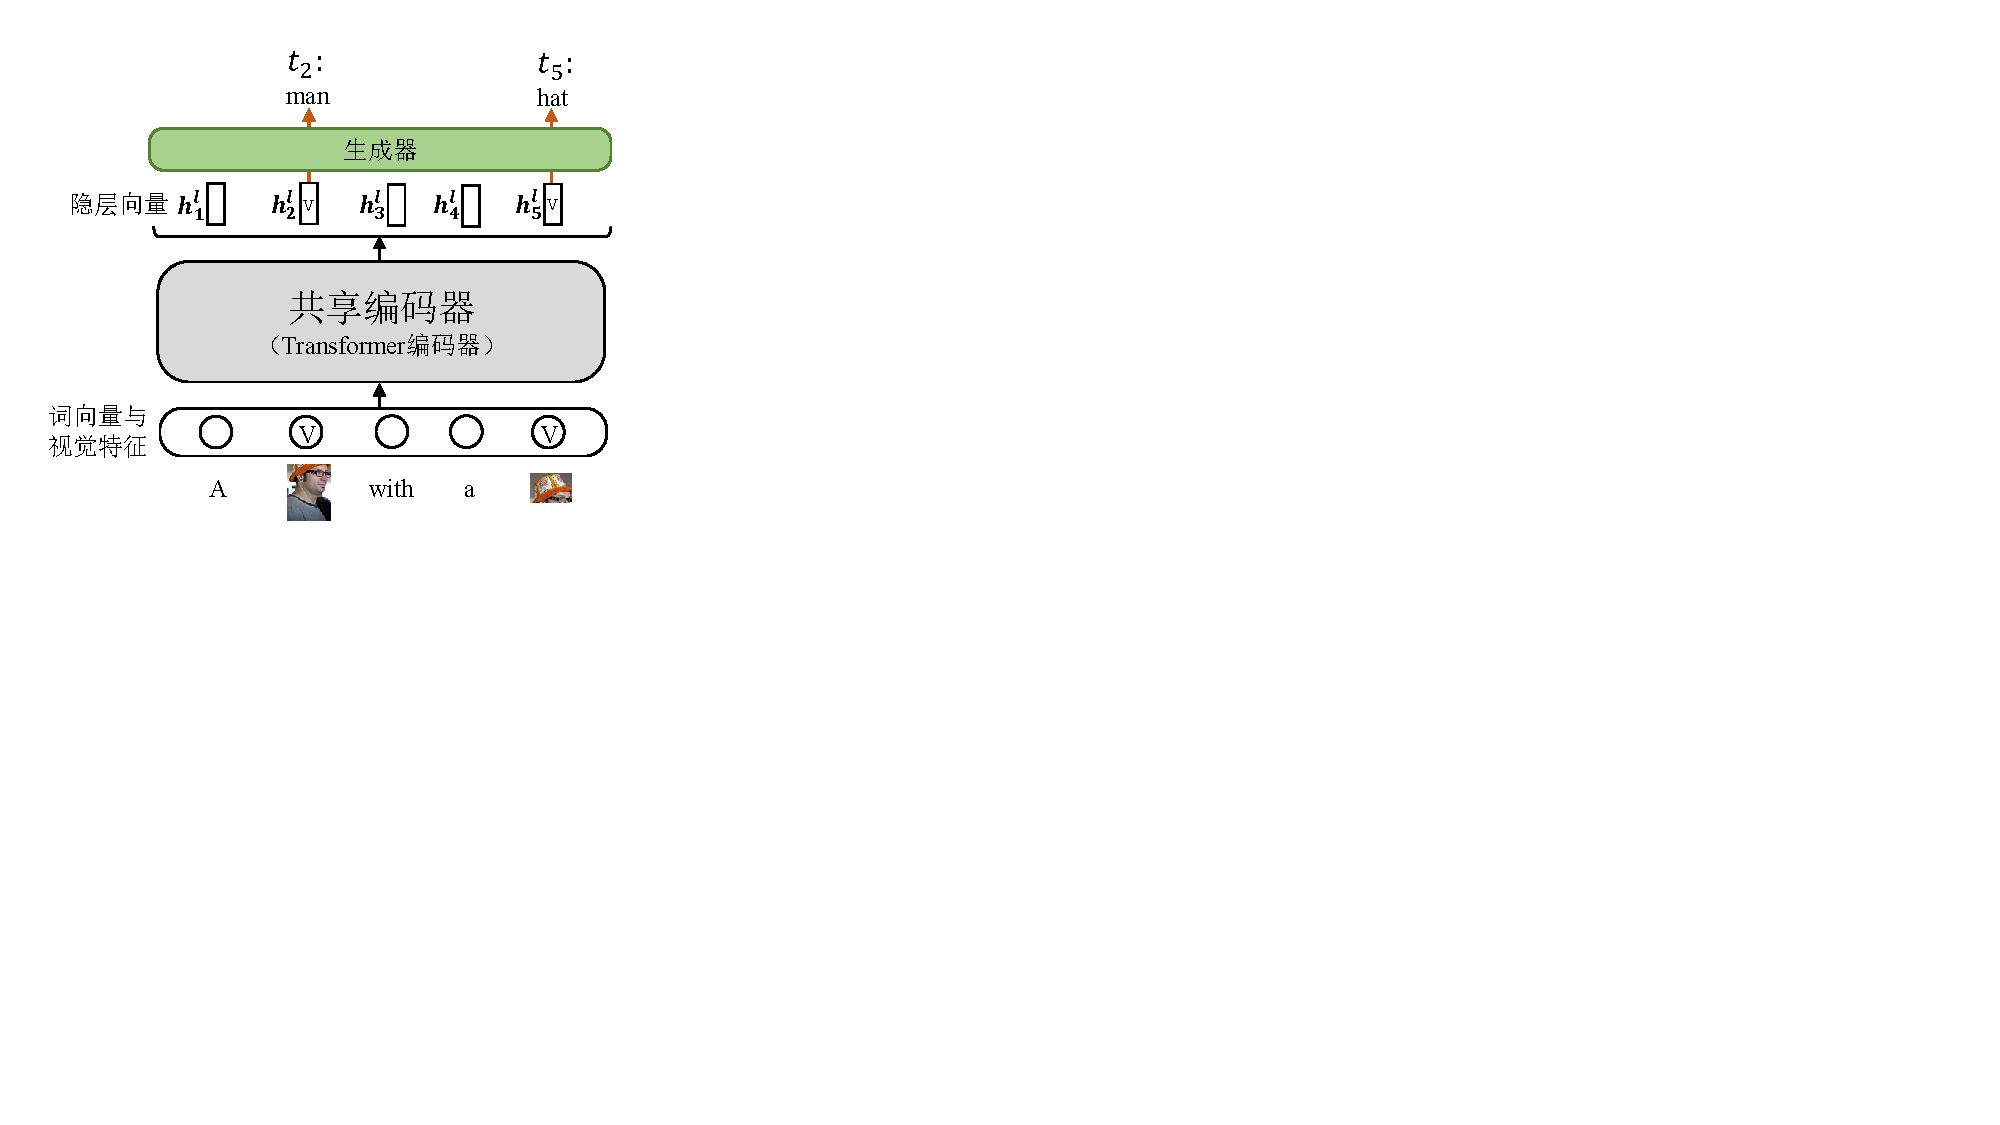
\includegraphics[scale=0.7]{Img/fig_4_ter.pdf}
    \bicaption{文本实体重构}{Textual entity reconstruction}
    \label{fig:4_ter}
\end{figure}
%(1){\sffamily 跨模态实体:}其中实体重构主要依赖于跨模态实体所提供的具体信息。如图【】所示,文本实体$t_1$的重构主要依赖于视觉实体$e_1$,视觉实体$e_1$的重构也主要依赖于文本实体$t_1$。

%\item
%(2){\sffamily 文本上下文:}本文所用文本上下文为经过退化的文本$\tilde{X}$。例如图【】中进行实体重构时,文本上下文为“A <M> with a <M>”,其中“<M>”代表将实体词所对应的位置删除并保留该位置空缺。文本上下文与跨模态实体共同组成文本的完整语义。在进行视觉实体重构时,模型的输入由文本上下文和文本实体共同组成,即原文本$X$。在进行文本实体重构时,模型的输入是文本上下文和视觉实体所组成的多模态混合序列$Z$。在进行文本非实体的重构时,模型的输入同样是多模态混合序列,但是需要将待重构的非实体词利用掩码词“<M>”替换掉,形成$\tilde{Z}$。跨模态实体与文本上下文组合重构实体的方式,既能保证重构实体时具备充足的语义信息,又能充分利用到自注意力机制的特性使实体与文本上下文建立良好的语义关系。

%\item
%(3){\sffamily 实体对齐关系:}为了避免让模型完成较为困难的跨模态实体关系对齐,本文采用直接替换对应位置向量表示的方式。例如图2中重构文本实体$t_1$时,将输入序列中的对应位置直接替换为视觉实体的向量表示${\boldsymbol{e}_1}$。

\subsection{跨模态实体重构}
\label{sec:4_cer}
\begin{figure}[!htbp]
    \centering
    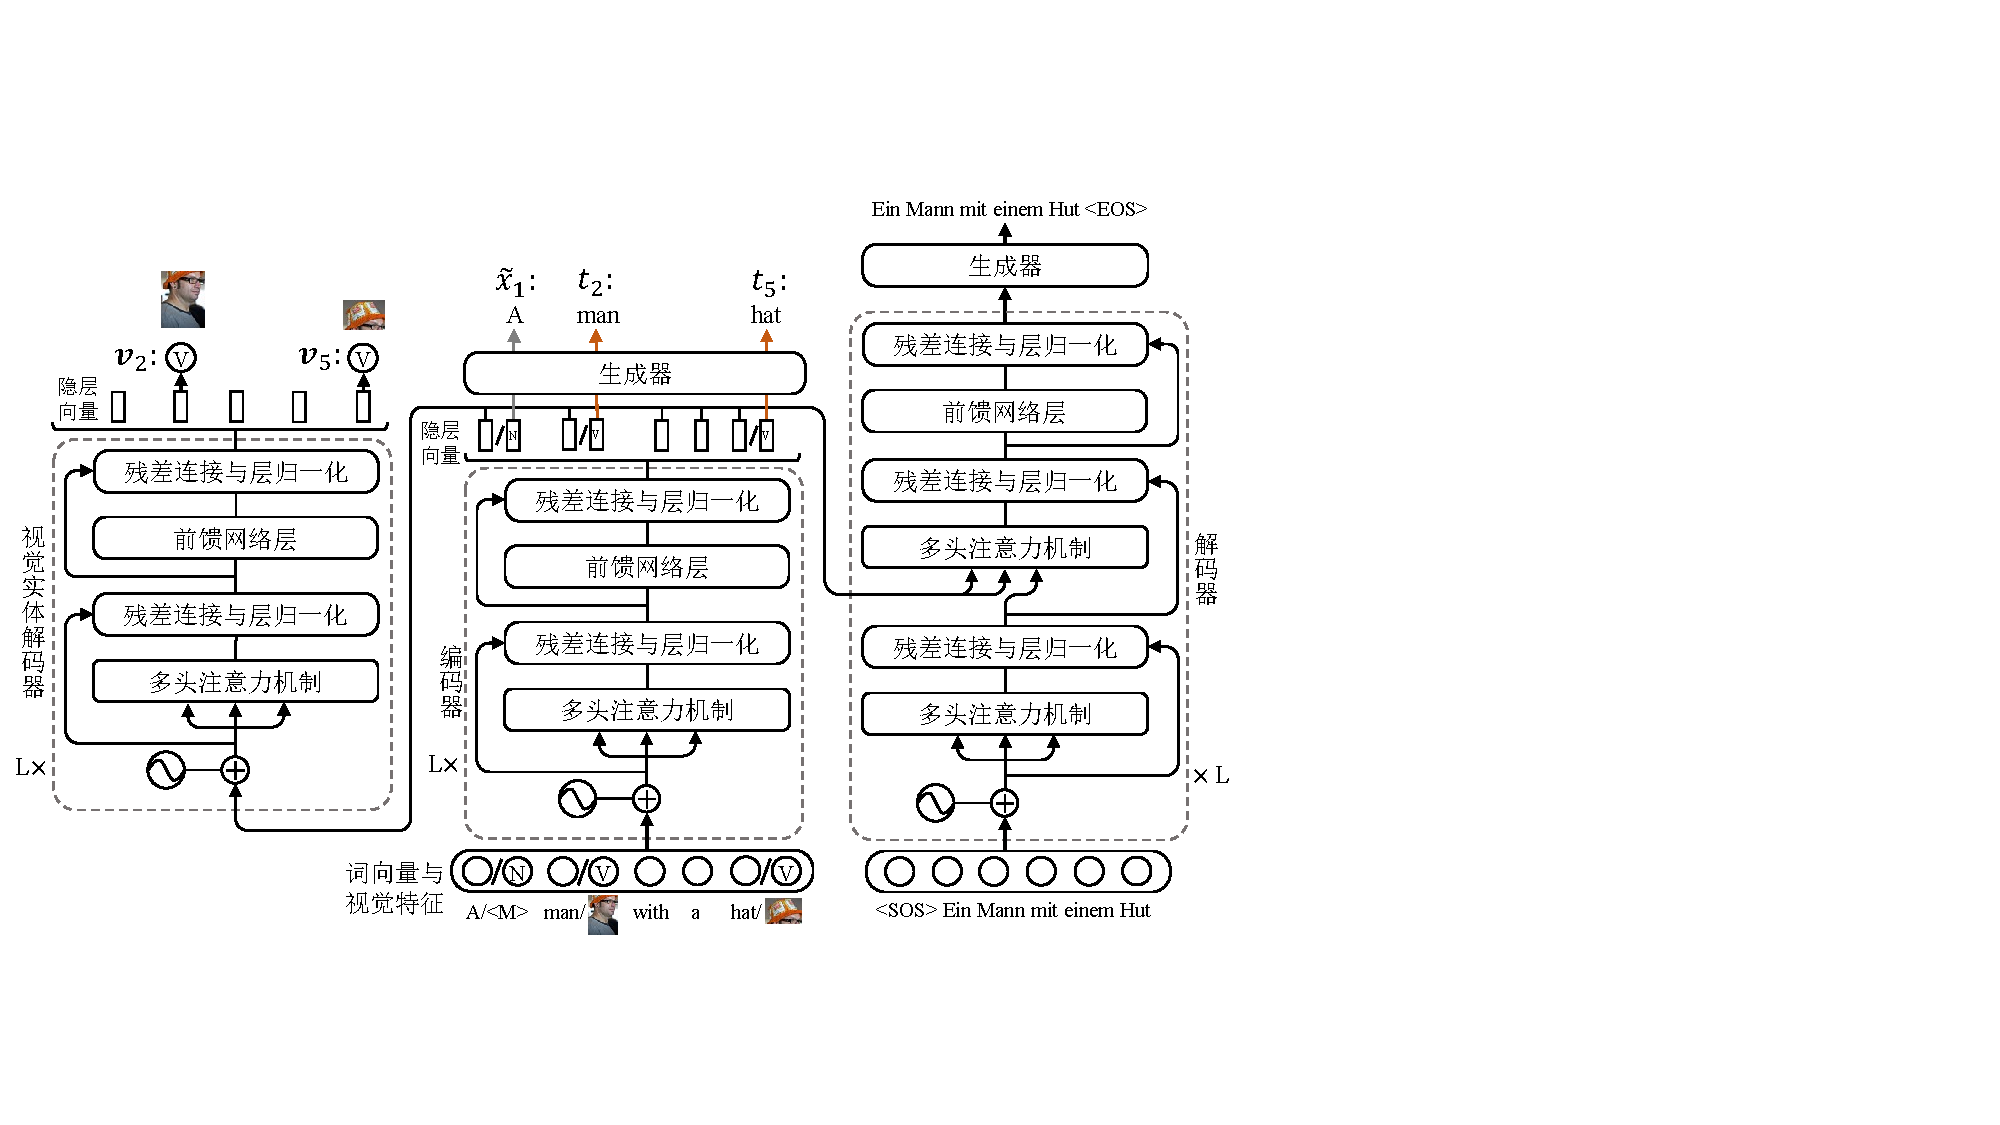
\includegraphics[scale=0.65]{Img/fig_4_model.pdf}
    \bicaption{结合跨模态实体重构方法的神经机器翻译}{NMT model framework combined with CER}
    \label{fig:4_model}
\end{figure}
图\ref{fig:4_model}展示了CER模型与NMT模型相融合的简化过程,其中包含了视觉实体解码器、跨模态编码器以及翻译解码器三个主要组成部分。其中最核心的跨模态编码器负责在实体重构之前将视觉信息与文本信息编码融合。解码器仅用于主任务翻译的目标文本解码。视觉实体解码器负责将跨模态编码器编码后的状态解码到视觉目标所代表的视觉语义空间,而其结构与编码器相同均为$L$层Transformer编码器。为了更详细地介绍CER方法是如何工作的,以及如何与神经机器翻译相结合,本节将CER方法分为:文本实体重构、视觉实体重构以及文本非实体重构三个子任务进行详细的介绍。

{\sffamily (1)文本实体重构}

\begin{figure}[!htbp]
    \centering
    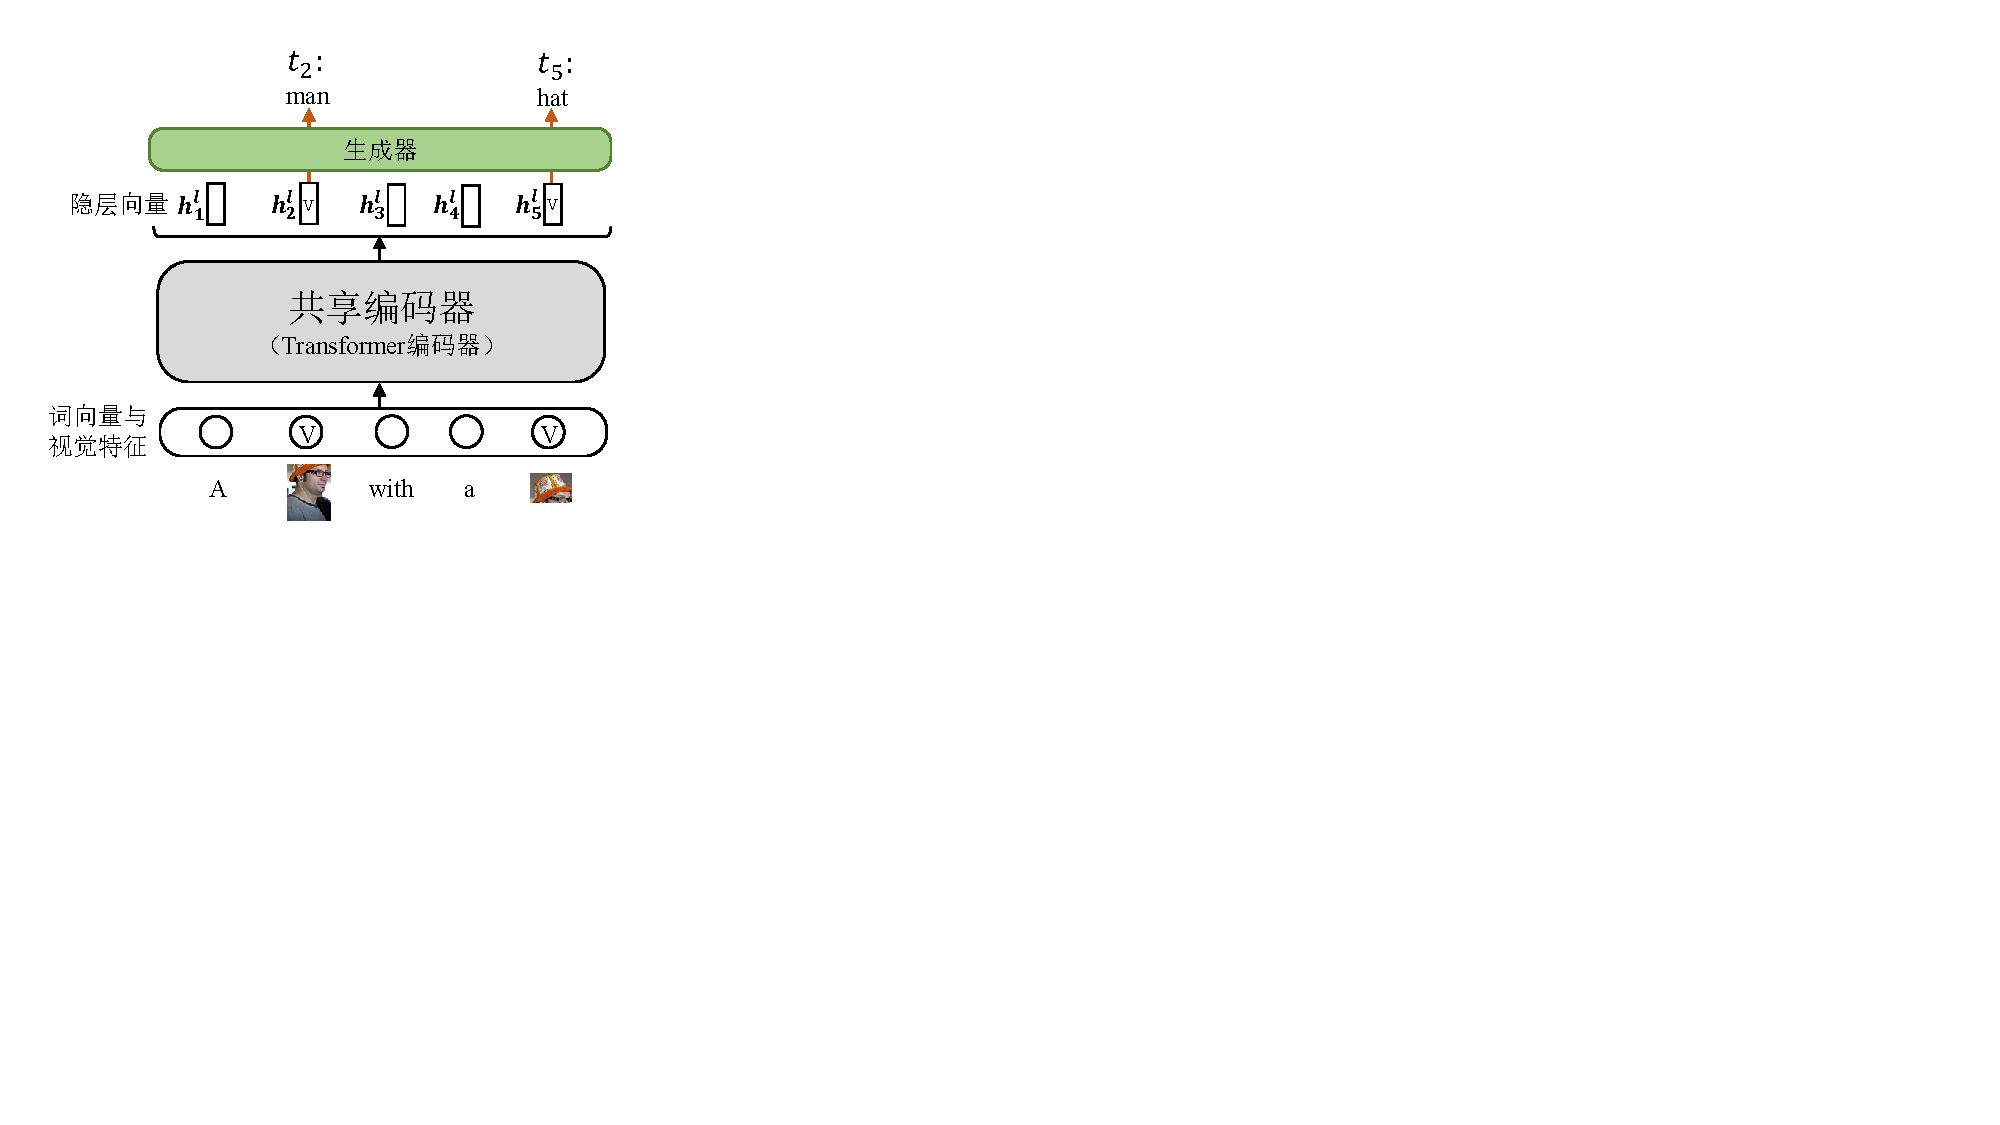
\includegraphics[scale=0.7]{Img/fig_4_ter.pdf}
    \bicaption{文本实体重构}{Textual entity reconstruction}
    \label{fig:4_ter}
\end{figure}
文本实体重构(textual entity reconstruction,TER)与上一章相似,将视觉目标明确地作用到文本实体上。本章仅针对有对应视觉目标的名词采取实体替换,因此文本实体重构的输入为由文本上下文$\tilde{X}$和视觉实体$V$组合成的多模态混合序列:
\begin{equation}
Z={\rm{Combine}} \left( \tilde{X}, V \right)
\end{equation}
如图\ref{fig:4_ter}所示,输入的文本上下文“A <mask> with a <mask>”与视觉实体$\{v_2,v_5\}$组合成多模态混合序列$Z=$“A $v_2$ with a $v_5$”,此时输入到模型中的是三个空心圆代表的词向量和两个标记“V”的圆代表的$v_2$和$v_5$对应的视觉特征。跨模态混合序列经过编码器进行跨模态编码后,得到序列的跨模态表示:
\begin{equation}
\Vector{H_Z^L}={\rm{MultiHead_{enc}^L}} \left( Z, Z, Z \right)
\end{equation}
其中,$\Vector{H_Z^L}=\{\Vector{h_1^l,h_2^l,\cdots,h_N^l}\}$;${\rm{MultiHead_{enc}^L}} \left( \cdot,\cdot,\cdot \right)$代表$L$层采用多头注意力机制的编码器;$\Vector{h_i^l}$中的$l$与$L$相同,代表第$l$层的编码结果。然后依据对应位置的隐层表示生成文本实体,在图2中为两个标记“V”的矩形隐层表示${\Vector{h_2^l}}$和${\Vector{h_5^l}}$,该过程需要优化以下损失函数:
\begin{equation}
\mathcal{L}_{\rm{TER}} (\theta, \vartheta) =
    \frac{1}{{\vert}T{\vert}}
    \mathop{\sum}_{x_i \in T}
    {\rm{OH}} \left( x_i \right)
    {\rm log}{\ }{\rm p} \left( Z {\vert} \theta, \vartheta \right)
\end{equation}
\begin{equation}
{\log}{\ }{\rm p} \left( Z {\vert} \theta, \vartheta \right) =
    {\rm{g}} \left( \Vector{h_i^l} \vert \vartheta \right)
\end{equation}
其中${\rm{OH}}\left(x_i\right)$代表$x_i$的独热编码(One-hot,OH)表示,$\theta$代表编码器一端的参数,$\vartheta$为生成器(generator)参数,生成器${\rm{g}}\left(\cdot\right)$将位置$i$处的隐层向量${\Vector{h_i^l}}$映射并得到词表中每个词的预测概率。

{\sffamily (2)视觉实体重构}

\begin{figure}[!htbp]
    \centering
    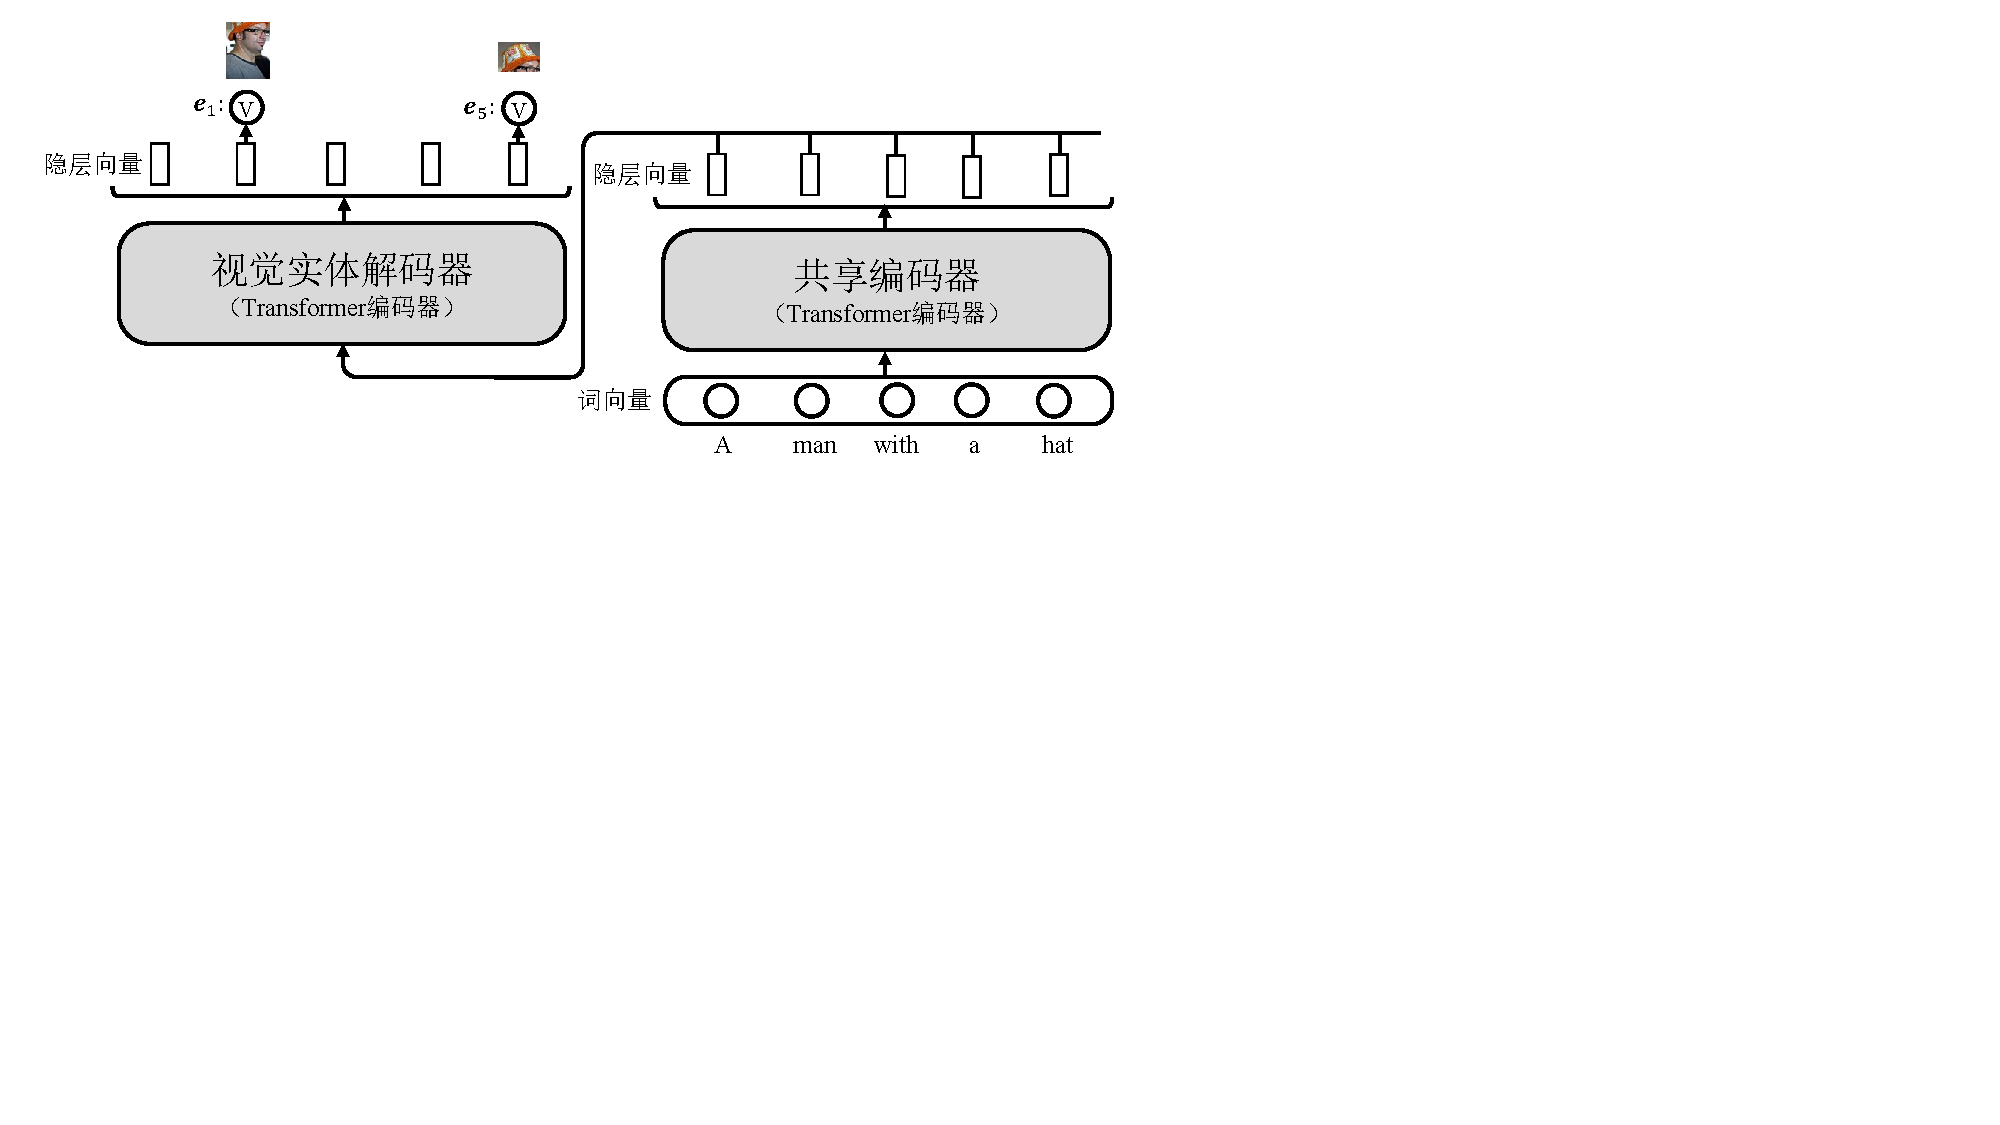
\includegraphics[scale=0.6]{Img/fig_4_ver.pdf}
    \bicaption{视觉实体重构}{Visual entity reconstruction}
    \label{fig:4_ver}
\end{figure}
与文本实体重构不同的是,视觉实体重构(visual entity reconstruction,VER)依赖于来自单一文本模态的$X$。例如图\ref{fig:4_ver}中,“A man with a hat”是重构视觉实体时模型的输入序列,此时图中输入到模型中的是5个空心圆代表的词向量。该句子经过$L$层的编码器进行文本编码,再利用$L$层视觉实体解码器解码出与文本实体$\{t_2,t_5\}$相对应的视觉实体$\{v_2,v_5\}$。由于文本无法完整的描述图片,只是针对图片中的个别属性的描述,由文本直接还原像素级的图片或图片中的视觉实体几乎是不可能的。因此本文仅尝试生成与视觉实体相近的向量表示$\{\Vector{v_2,v_5}\}$。其中,$X$经过如下编码过程:
\begin{equation}
\Vector{H_X^L}={\rm{MultiHead_{enc}^L}}(X, X, X)
\end{equation}
得到编码后的隐层表示$\Vector{H_X^L}=\{\Vector{h_1^l,h_2^l,\cdots,h_N^l}\}$。然后经过如下解码过程:
\begin{equation}
\Vector{H_X^{2L}}={\rm{MultiHead_{dec}^L}}(\Vector{H_X^L, H_X^L, H_X^L})
\end{equation}
得到$\Vector{H_X^{2L}}=\{\Vector{h_1^{2l},h_2^{2l},\cdots,h_N^{2l}}\}$,${\rm MultiHead_{dec}^L}\left( \cdot,\cdot,\cdot \right)$为与${\rm MultiHead_{enc}^L}\left( \cdot,\cdot,\cdot \right)$具有相同结构的视觉实体解码器。然后利用$\Vector{H_X^{2L}}$生成与$\{\Vector{v_a,v_b,\cdots}\}$接近的向量表示,文本采用与\tcite{elliott2017imagination}相近的方式实现该过程:
\begin{equation}
\mathcal{L}_{\rm{VER}}(\theta, \varphi)=
    \frac{1}{{\vert}V{\vert}}
    \mathop{\sum}_{i \neq j}{\max}\{0, \varepsilon - {\rm{cos}}\left( \Vector{h_i^{2l}}, \Vector{v_j} \right) + {\rm{cos}}\left( \Vector{h_i^{2l}}, \Vector{v_i} \right)\}
\end{equation}
%\onecolumn
%\input{docs/model_pic.tex}
%\begin{multicols}{2}
其中$i=a,b,\cdots$为实体在句子中对应的序号;$\varphi$为视觉实体解码器的参数;${\rm{cos}}(\cdot,\cdot)$计算向量间的余弦相似度,$\varepsilon$为最小边缘常量。显然,优化$\mathcal{L}_{\rm{VER}}(\theta,\varphi)$能够缩减$\Vector{h_i^{2l}}$与相对应的视觉实体$\Vector{v_i}$之间的余弦距离,增加与其它非对应的视觉实体$\Vector{v_j}$之间的余弦距离。

{\sffamily (3)文本非实体重构}

\begin{figure}[!htbp]
    \centering
    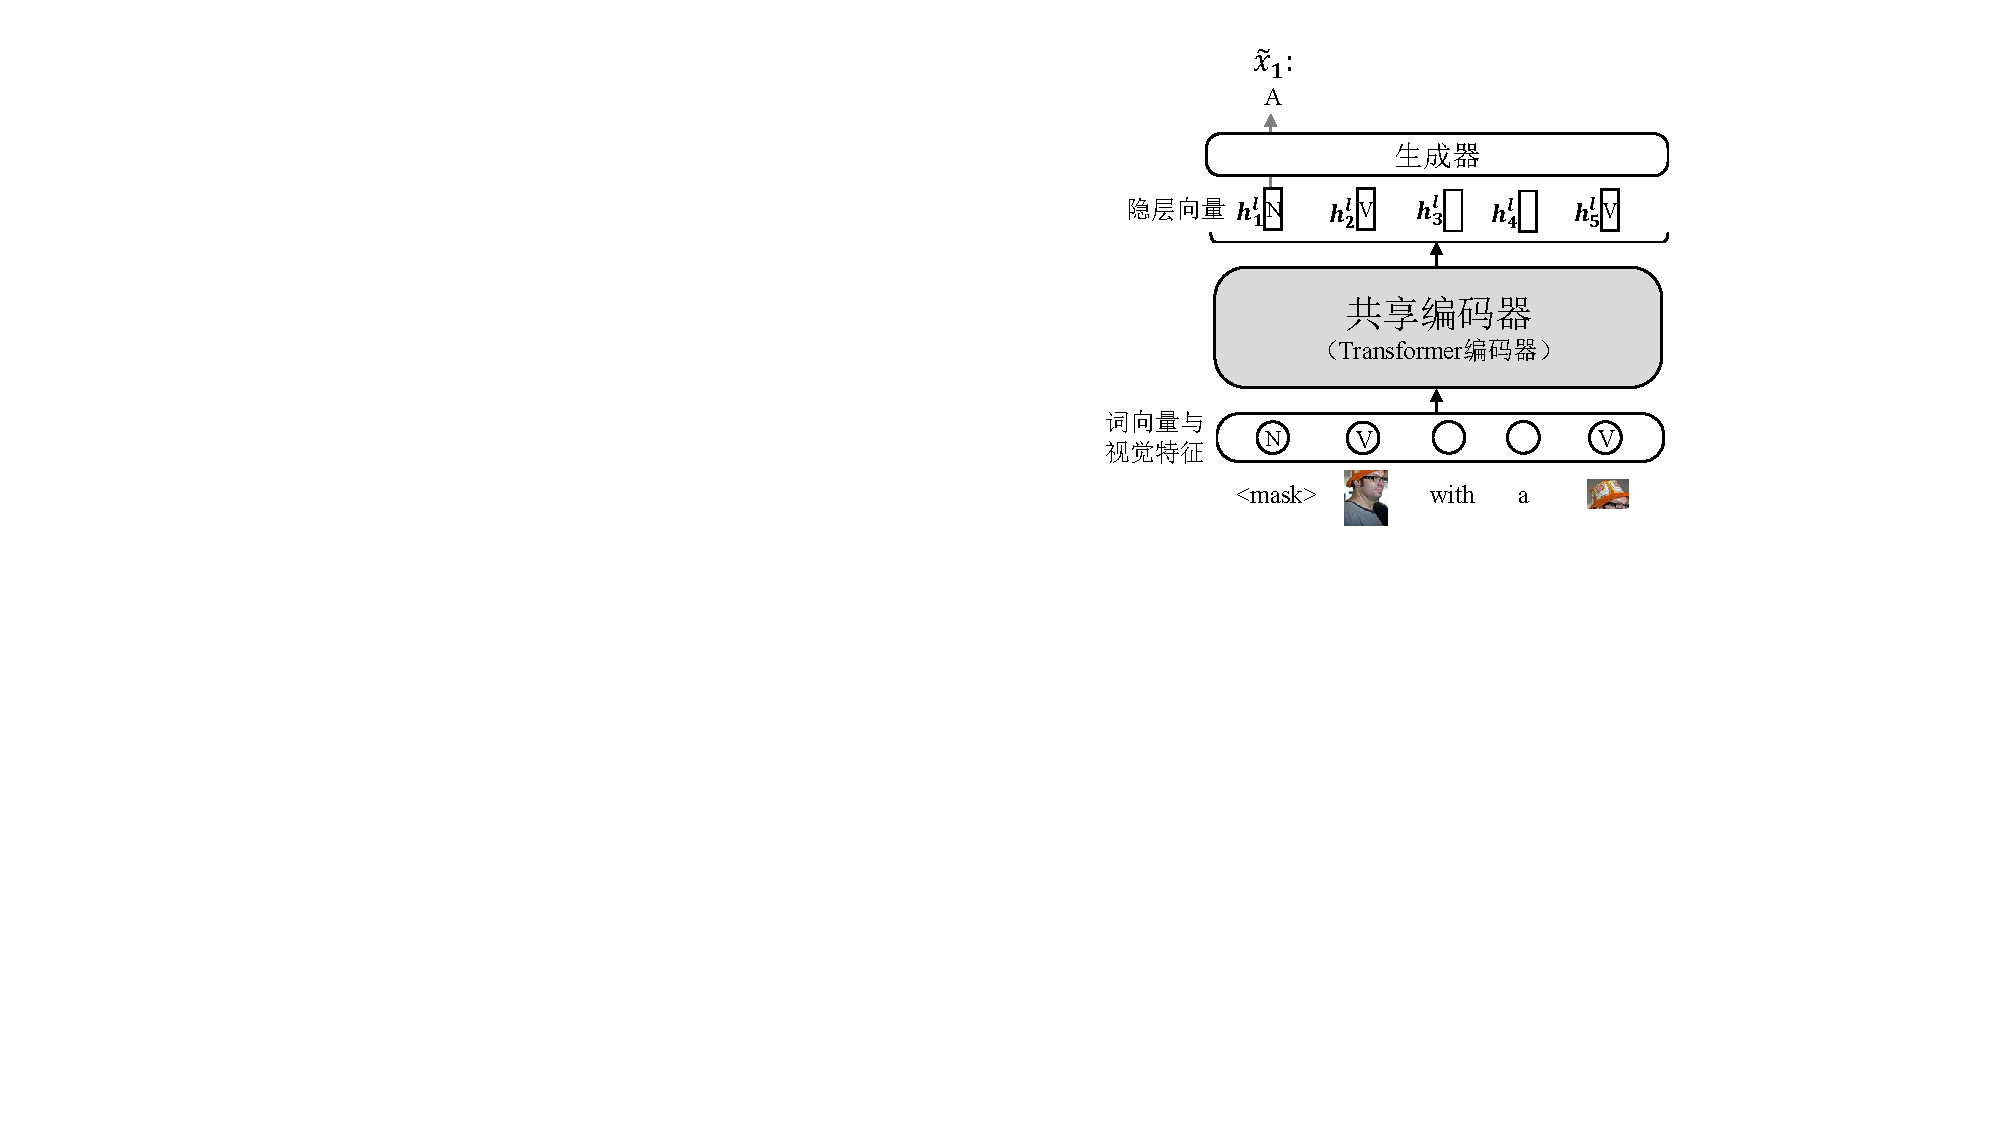
\includegraphics[scale=0.6]{Img/fig_4_tner.pdf}
    \bicaption{文本非实体重构}{Textual none-entity reconstruction}
    \label{fig:4_tner}
\end{figure}
文本非实体重构(textual none-entity reconstruction,TNER)方法与文本实体重构方法相似,区别在于非实体重构的目的是使视觉实体与文本上下文进行充分的句子级语义融合,而实体的重构方法更侧重实体在两个模态之间的实体级语义融合。文本非实体的输入同样是文本上下文$\tilde{X}$和视觉实体$V$组合成的多模态混合序列,但是在$\tilde{X}$中除对实体的位置进行退化还要将待重构的非实体词退化。例如图\ref{fig:4_tner}中,当选择对非实体词“A”进行重构时,模型所输入的跨模态混合序列为$\tilde{Z}=$“<mask> $v_2$ with a $v_5$”,此时输入到模型中的是一个标记“N”的圆形,代表“<mask>”的词向量,以及两个空心圆形所代表的词向量和两个标记“V”的圆形所代表的视觉特征。损失函数如下:
%一个标记``N''的圆形词向量代表``$\langle$M$\rangle$''、两个圆形空心词向量和两个标记``V''的圆形视觉特征. 损失函数如下:
\begin{equation}
\mathcal{L}_{\rm{TNER}}(\theta, \vartheta) =
    \frac{1}{{\vert}\tilde{T}{\vert}}
    \mathop{\sum}_{x_i \in \tilde{T}}
    {\rm{OH}} \left( x_i \right)
    {\rm log}{\ }{\rm p} \left( \tilde{Z} {\vert} \theta, \vartheta \right)
\end{equation}
其中$\tilde{T}$代表待重构的非实体词集,并有$\tilde{T}\subseteq \tilde{X}$。在图2中用于预测非实体词“A”的隐层为一个标记“N”的矩形隐层表示$\Vector{h_1^l}$。

本文采用随机选取的方式在句子中选择待重构的非实体词。在执行TNER任务时,每个文本中的非实体词有$30\%$的概率会被选择到。该概率与所采用数据集中实体词占$32.6\%$的比例相近。

{\sffamily (4)CER联合训练}

联合以上所有重构方法的目标函数,可得到本章所提CER方法的联合损失函数为:
\begin{equation}
\mathcal{L}_{\rm{CER}} \left( \theta, \varphi, \vartheta \right) = \alpha \mathcal{L}_{\rm{VER}} \left( \theta, \varphi \right) + \beta \mathcal{L}_{\rm{TER}} \left( \theta, \vartheta \right) + \gamma \mathcal{L}_{\rm{TNER}} \left( \theta, \vartheta \right)
\label{eq:4_combined_cer}
\end{equation}
其中,$\alpha$、$\beta$和$\gamma$为控制三种重构方法训练比例的超参数。值得注意的是,本章没有设置利用纯文本上下文$\tilde{X}$重构文本词的方案。这是因为该方案与一般的预训练方法相似,用于建立纯文本的语言模型。而机器翻译模型的编码端本身就是一个很好的纯文本语言模型,因此不必再设置纯文本的重构方案。

\subsection{与机器翻译相结合}
构建CER模型的目的是辅助翻译模型提升翻译质量。本章采用多任务训练方法将CER方法中的跨模态编码器与神经翻译模型的文本编码器进行参数共享,从而实现对神经机器翻译模型参数优化的目的。翻译任务所要优化的目标函数为:
\begin{equation}
\mathcal{L}_{\rm{NMT}} \left( \theta, \phi \right) =
    -\mathop{\sum}_j^M {\rm log}{\ }{\rm P} \left(y_j \vert y_{<j}, X \vert \theta, \phi \right)
\label{eq:4_nmt}
\end{equation}
其中$Y=\{y_1,y_2,\cdots,y_M\}$为目标语言的文本序列;$\phi$为解码器一端的参数,值得注意的是,在文本实体重构与文本非实体重构中所应用的生成器参数$\vartheta$是$\phi$的一部分,即采用的是同一个生成器。将公式(\ref{eq:4_nmt})与CER模型的损失函数公式(\ref{eq:4_combined_cer})相结合得到联合目标函数为:
\begin{equation}
\mathcal{L} \left( \theta, \phi, \varphi \right) = \omega\mathcal{L}_{\rm{NMT}} \left( \theta, \phi \right) + \left( 1-\omega \right) \mathcal{L}_{\rm{CER}} \left( \theta, \varphi, \vartheta \right)
\end{equation}
其中,用超参数$\omega$调节神经机器翻译与CER方法的训练比例。